\chapter{行を消す}
\section{盤面をどのように表現しているかのおさらい}
盤面は、self.boardに2次元リスト、つまりリストが入っているリストとして保存されています。
「リストのリスト」は下のようなイメージです。
\begin{figure}
  [h]
  \centering
  \includegraphics[width=50mm, page=25]{images/Elements.pdf}
  \caption{リストのリスト}
\end{figure}
このリストの0番目は、0行目のデータを表しています。
リストの0番目の4番目(=[0][4])は、(4,0)のデータを表しています。
最初が行(Y座標)、次が列(X座標)です。
\section{盤面を確認して行を消す関数erase\_lines}
盤面を確認して、揃った行を消す関数erase\_linesを作ります。
\subsection{リストに特定の要素があるかどうか}
リストに特定の要素があるかどうかを調べるには、inを使います。
今回はBLACKが入っていないなので、さらにその否定であるnotを使いましょう。
\begin{lstlisting}[caption=リストに特定の要素があるかどうか,label=sample, language=Python]
if not BLACK in self.board[y]:
    # その行を消す
\end{lstlisting}
これを全てのyに対して行います。
\subsection{行を消す操作}
復習になりますが、リストから要素を消すにはpop(番号)を使います。
\begin{lstlisting}[caption=リストから要素を消す,label=sample, language=Python]
  num_list = [1,2,3,4,5]
  num_list.pop(2) # num_listは[1,2,4,5]になる
\end{lstlisting}
2の要素を消すのではなく、あくまで2番目の要素を消すことに注意してください。
また、行を消した後、上から空の行を追加することで、盤面全体行数が変わらないようにします。
リストの先頭に要素を追加するにはinsert(番号, 要素)を使います。
先頭の番号は0なので、今回はinsert(0, 要素)という形になるはずです。
\begin{lstlisting}[caption=新たな行を追加,label=sample, language=Python]
  num_list = [1,2,3,4,5]
  num_list.pop(2) # num_listは[1,2,4,5]になる
  num_list.insert(0, 0) # num_listは[0,1,2,4,5]になる
\end{lstlisting}

\subsection{erase\_linesの実装}
以下のコードを追加して、erase\_linesを実装しましょう。
\lstinputlisting[caption={行を消す関数erase\_lines}, language=Python]{chapter11/ch11_1_1.py}

\section{erase\_linesを呼び出す}
行を消すタイミングは、ブロックが固定された後が適しています。
ブロックを固定する関数は、前回作ったfix関数なので、ここに書き足します。
\lstinputlisting[caption={erase\_linesの呼び出し}, language=Python]{chapter11/ch11_2_1.py}
うまく消えたことが確認できたら終わりです。